\section{Onboard Gate Perception and Target Association}
\label{sec:perception}

A racing benchmark is only meaningful if target selection remains part of the
participant's autonomy problem. The observation contract of
Section~\ref{sec:obs_contract} does not expose ground-truth gate geometry or
referee progress, while the forward camera may contain several gates and the
acoustic channel may simultaneously deliver packets from several transmitters.
The received packets do not indicate which beacon is currently relevant; that
state is maintained locally by the controller. Selecting which visible gate
corresponds to the locally expected beacon must therefore be performed onboard
rather than by the benchmark.

The reference perception front end combines geometric detection in the forward
camera with acoustic target association, as summarized in
Fig.~\ref{fig:perception_pipeline}. The visual stage produces multiple candidate
gates rather than a single preselected target, while the acoustic stage provides
bearing and range information for the beacon expected by the controller. Their
combination produces either one visual target or no visual target for the
current frame.

\begin{figure}[t]
\centering
\scriptsize
\begin{tikzpicture}[
  node distance=0.42cm,
  box/.style={draw, rounded corners=2pt, fill=mralight, align=center,
    text width=2.35cm, minimum height=0.72cm, inner sep=3pt},
  acou/.style={draw, rounded corners=2pt, fill=white, align=center,
    text width=2.35cm, minimum height=0.72cm, inner sep=3pt},
  arrow/.style={-Latex, thick},
  lbl/.style={font=\tiny}
]
\node[box] (cam) {FrontCamera\ RGB image};
\node[box, right=of cam] (edge) {grayscale\ + Canny};
\node[box, right=of edge] (cont) {closed contours\ + bounding boxes};
\node[box, right=of cont] (filt) {geometric filter\ size, aspect, $\Pi$, $\alpha$};
\node[box, below=0.75cm of filt] (cands) {candidate list\ $(c_x,c_y,\alpha,\gamma)$, top 8};
\node[acou, left=of cands] (assoc) {association\ FOV, bearing, size gates};
\node[acou, left=of assoc] (beacon) {expected-beacon\ packet $(\beta,\tilde\rho)$};
\node[box, left=of beacon] (out) {visual target\ or \emph{none}};

\draw[arrow] (cam) -- (edge);
\draw[arrow] (edge) -- (cont);
\draw[arrow] (cont) -- (filt);
\draw[arrow] (filt) -- (cands);
\draw[arrow] (cands) -- (assoc);
\draw[arrow] (beacon) -- (assoc);
\draw[arrow] (assoc) -- (out);
\end{tikzpicture}
\caption{The onboard gate-perception front end. Camera pixels produce an
unlabelled candidate list; the controller's own expected-beacon packet supplies
the bearing that selects among them. No simulator gate pose, global vehicle pose
or referee target enters any stage.}
\label{fig:perception_pipeline}
\end{figure}



\subsection{Gate Detection from the Forward Camera}
\label{sec:perception_detect}

The gates are rendered as square frames formed by light-coloured bars. Direct
colour or brightness segmentation is unreliable because underwater rendering
can substantially alter their apparent intensity relative to the water and
seabed. The detector therefore relies primarily on geometric structure: edges
are extracted from the grayscale image, closed contours are converted into
bounding boxes, and candidates are filtered according to their apparent size,
aspect ratio and consistency with a rectangular frame. These criteria are fixed
for the evaluation and are applied unchanged across the three official
circuits.

For an image of width $W$ and height $H$, the centre of a surviving candidate
is expressed in normalized image coordinates as
\begin{equation}
\label{eq:vision_center}
c_x=
\frac{(x+\tfrac{1}{2}w_{\mathrm{px}})-\tfrac{1}{2}W}
{\tfrac{1}{2}W},
\qquad
c_y=
\frac{(y+\tfrac{1}{2}h_{\mathrm{px}})-\tfrac{1}{2}H}
{\tfrac{1}{2}H}.
\end{equation}
Here $(c_x,c_y)$ is the displacement of the candidate centre from the optical
axis, while its apparent size is represented by the image-area fraction
$\alpha$. Each candidate is also assigned a confidence $\gamma$ that combines
shape consistency, aspect-ratio plausibility, apparent size and image
centredness. A single fixed parameter set is used for all official circuits;
the exact thresholds and weights are provided with the released implementation.

The detector retains multiple plausible candidates and removes near-duplicate
detections before passing the resulting ranked list to the association stage.
Retaining several candidates is important in the racing setting because
consecutive gates can be simultaneously visible; a visual detector that selected
a single rectangle by itself would implicitly solve part of the
course-association problem.


\subsection{Acoustic--Visual Target Association}
\label{sec:perception_assoc}

The controller maintains its own locally expected beacon
(Section~\ref{sec:controller}). When a packet from that beacon is available, it
provides a noisy bearing $\beta$ and measured range $\tilde{\rho}$ according to
the acoustic model of Section~\ref{sec:configuration}. The perception problem is
then to determine which, if any, of the visual candidates is geometrically
consistent with that acoustic observation.

The conceptual association path is shown in
Fig.~\ref{fig:schematic_perception}.
\begin{figure}[t]
\centering
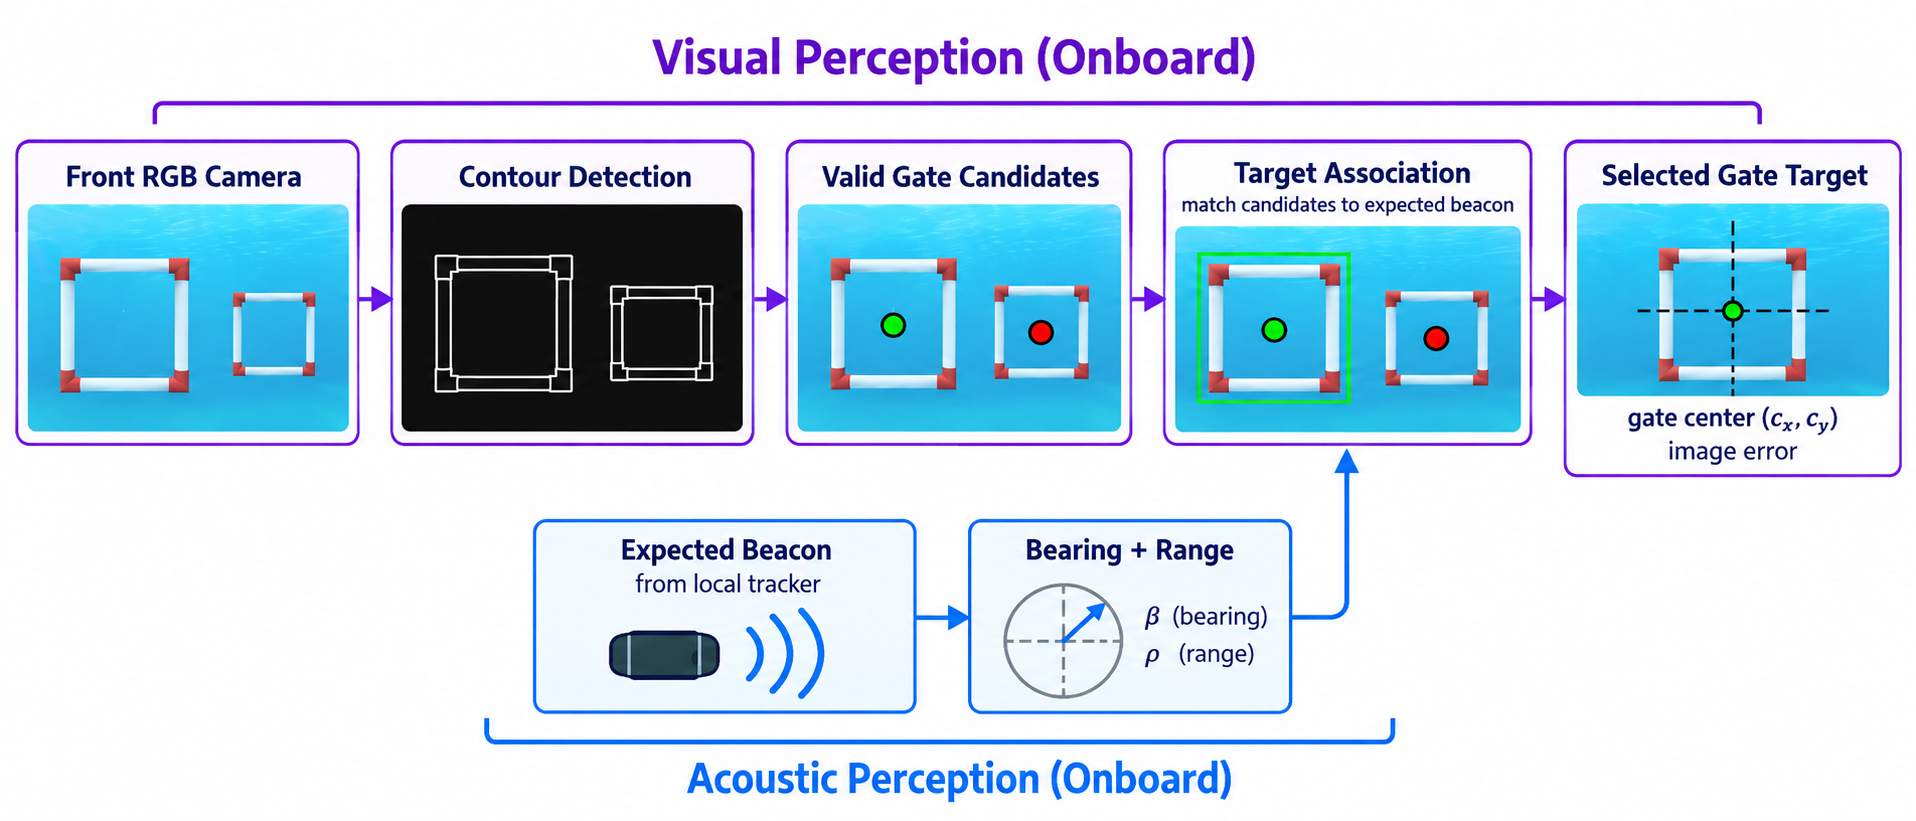
\includegraphics[width=\linewidth]{figures/p2.png}
\caption{Conceptual onboard perception path from camera and acoustic-channel
observations to candidate gates, beacon association and the selected target.}
\label{fig:schematic_perception}
\end{figure}


Association first rejects candidates that are inconsistent with the camera field
of view and the acoustic bearing. The horizontal image position of each
candidate provides an approximate visual bearing, which can be compared with
$\beta$. Apparent target size is also used as a consistency check at short range:
a nearby expected gate should occupy a substantial portion of the image, whereas
a small complete rectangle is more likely to belong to a farther gate.

When the acoustic bearing provides a clear directional constraint, candidates
that strongly disagree with it are rejected. The remaining detections are
ranked using visual confidence, image centredness, relative apparent size and
acoustic--visual bearing consistency. Relative rather than purely absolute size
is used so that a farther but visually centred gate does not systematically
dominate a closer candidate. The same association parameters are used throughout
the official circuits.

If no packet from the locally expected beacon is currently available, the
association falls back to visual evidence and favours large, confident and
well-centred candidates. If no candidate remains plausible, no visual target is
returned and the controller continues using the other onboard measurements.

This design preserves the benchmark information boundary. Target association
depends only on the controller's local course state, camera detections and
received acoustic measurements. It does not use simulator gate poses, the global
vehicle pose or the referee's expected-gate index. An incorrect association is
therefore an autonomy error rather than an error hidden by benchmark-side target
selection.


\subsection{Exploratory Pose-Aware Extension}
\label{sec:perception_pose}

The centre-based representation does not describe the orientation of the gate
plane. We therefore also implemented a pose-aware variant that uses a detected
aperture quadrilateral together with the known nominal gate aperture to estimate
relative plane orientation and distance.

Its behaviour is strongly dependent on viewing geometry. In a dedicated set of
oblique views, a valid pose estimate was obtained in only $11.7\%$ of frames and
the median plane-yaw error was $48.2^\circ$. The estimator is therefore
unreliable under large oblique viewing angles, motivating the separate
characterization under the viewing conditions encountered during normal racing.


\subsection{Perception Audit on the Official Circuits}
\label{sec:perception_audit}

To characterize perception under the conditions encountered by the reference
controller, we recorded 60 frames per circuit along its trajectories on the
three official circuits. Ground truth was used only offline to evaluate the
perception output and never entered the control loop. Table~\ref{tab:perception_audit}
summarizes detection availability, quadrilateral recovery, pose availability and
multi-candidate target association, while
Fig.~\ref{fig:perception_panels} shows representative states.

\begin{table}[t]
\centering
\caption{Onboard perception audit on the official circuits.}
\label{tab:perception_audit}
\mratablestyle
\begin{tabular}{@{}lrrrrrrrr@{}}
\toprule
 & \multicolumn{3}{c}{Availability} & \multicolumn{3}{c}{Plane orientation error} & \multicolumn{2}{c}{Association} \\
\cmidrule(lr){2-4}\cmidrule(lr){5-7}\cmidrule(l){8-9}
Circuit & Det. & 4-corner & PnP & med.\ ($^{\circ}$) & p90 ($^{\circ}$) & $>\!30^{\circ}$ & multi & correct \\
\midrule
Horseshoe Bay    & 0.900 & 0.817 & 0.517 & 0.018 & 1.204 & 0.000 & 7  & 1.000 \\
Vertical Serpent & 0.883 & 0.783 & 0.483 & 1.129 & 4.287 & 0.000 & 4  & 1.000 \\
Mixed Endurance  & 0.917 & 0.833 & 0.533 & 0.064 & 0.064 & 0.000 & 11 & 1.000 \\
\bottomrule
\end{tabular}
\mratablenote
\emph{Det.}: fraction of frames with at least one accepted detection.
\emph{4-corner}: fraction with a validated aperture quadrilateral.
\emph{PnP}: fraction with a metric planar-PnP solution.
\emph{multi}: number of frames in which more than one candidate was present.
\emph{correct}: fraction of multi-candidate frames whose online association agreed
with an offline referee selection within a normalized centre tolerance of $0.25$;
the online target and the offline selection agreed on every frame of all three
circuits. No circuit recorded a wrong orientation sign, a gross orientation error
above $30^{\circ}$, a frame-to-frame yaw jump above $20^{\circ}$, or an
unintended online target switch. On Mixed Endurance the expected gate was outside
the field of view in $3$ of the $60$ frames; the in-view detection and four-corner
rates there are $0.912$ and $0.825$. This is a characterization of the perception
component from a diagnostic capture, not a controller performance claim.
\end{table}

\begin{figure}[t]
\centering
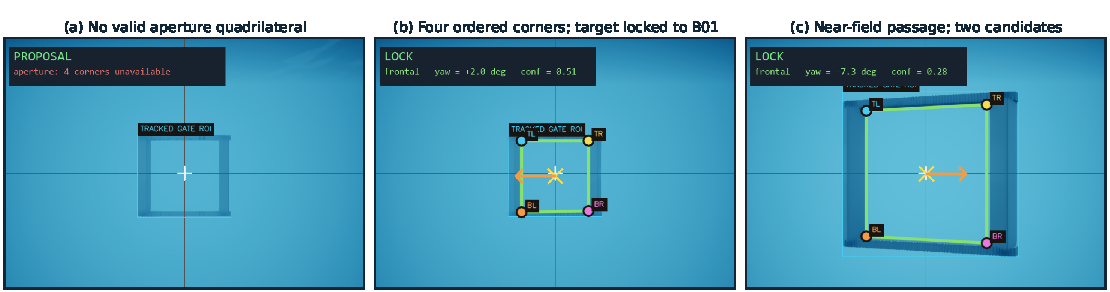
\includegraphics[width=\linewidth]{figures/generated/gate_perception_panels.pdf}
\caption{Onboard gate perception in the native HoloOcean simulator backend, one representative state per
official circuit. Each panel shows the forward-camera frame with the detector's
own overlays: the tracked aperture region, the four canonically ordered corners
(TL, TR, BR, BL), the image-centre crosshair, the estimated gate centre and the
image error vector of \eqref{eq:vision_center} that the visual servo drives to
zero. (a)~Mixed Endurance: a target is detected but no valid aperture
quadrilateral is available, so the front end degrades to the centre-only
estimate and reports an unknown orientation. (b)~Horseshoe Bay: four validated
corners with the target associated to the expected beacon \texttt{B01} at
$4.39$\,m and $-0.0^{\circ}$ bearing, tracker phase \textsc{visual\_align}.
(c)~Vertical Serpent: a near-field passage at $2.25$\,m with two raw candidates,
in which the association of Section~\ref{sec:perception_assoc} retains the
correct target, tracker phase \textsc{verify\_exit}. Nothing shown here is
derived from simulator gate poses or from the referee. Panel chrome from the
interactive viewer has been cropped and its state badge redrawn in English; the
detector overlays and all quoted values are unmodified.}
\label{fig:perception_panels}
\end{figure}


Detection was available in approximately $88$--$92\%$ of the recorded frames,
while a validated four-corner aperture was recovered in approximately
$78$--$83\%$. A metric pose estimate was available in roughly half of the
frames, confirming that pose recovery is substantially less reliable than
centre-based gate detection. The reference controllers are consequently designed
to tolerate intermittent visual measurements rather than assume that a complete
gate geometry is available at every control step.

Target association was considerably more stable. In every recorded frame
containing multiple visual candidates, the online association selected the same
gate as the offline reference: $7/7$ cases on Horseshoe Bay, $4/4$ on Vertical
Serpent and $11/11$ on Mixed Endurance. No unintended online target switch was
observed. This supports the use of acoustic bearing primarily as an identity cue
when several geometrically plausible gates are visible.

The pose results also clarify the difference between the dedicated oblique-view
test and normal racing. During the reference trajectories, the controller tends
to approach the gate approximately frontally. Under these conditions, the
recovered plane orientation was stable, with median yaw error below
$1.2^\circ$ on all three circuits and no gross orientation or sign errors
observed. Under strongly oblique views, by contrast, pose recovery became sparse
and inaccurate. The relevant conclusion is therefore not that the pose estimator
is generally reliable, but that its accuracy depends strongly on viewing
geometry.

For the racing task considered here, reliable gate-centre detection and
acoustic--visual association are sufficient for the reference controllers,
while full pose recovery is substantially more sensitive to viewpoint. The
perception audit characterizes these components independently from the
course-completion results reported in Section~\ref{sec:evaluation}.
